\section{Introduction}

\noindent
It's  a nice sunny day and you went for a picnic up a nice little mountain in Switzerland. You enjoyed your day and it t until you started your journey back when you noticed that the gas tank is almost empty. There are no gas stations around and that makes you worried until your friend says ``Never mind, we will use the force of gravity to accelerate us down''. Ahha! - you, being an avid student of physics, know exactl what your friend is talking about. Don't you?

\;
\noindent
In our everyday experience we know that objects are accelerated when moved by some force from one point to the other. This can be gravitational force or electromagnetic force.
We also know that higher the speed of an object, the more smashing energy it has. The damage to car moving with 5 mph in the parking lot is much less compared to the damage to a car on the highway when moving with a speed of 100 mph.

\;
\noindent
These two everyday observations are basic principles of particle accelerators - machines that accelerate very small particles to very high speeds and ''damage'' or break them either by smashing them into one another (like two cars head on) or on to a target (like a car colliding a wall). The difference is that the tiny paricles like protons, can be accelerated to very high speeds compared to a car on the highway. The Large Hadron Collider, the accelerator that discovered the Higgs boson just a couple years ago, can accelerate proton almost to the speed of light (v = 0.999999991*c = 299792455 m/s = 186282 miles/sec). The smashing power or energy of such particles on collision will not only break them, but, according to Einstein's famous E=mc2, part of this energy will actually turn into new particles. Imagine collision of two cars at a very high speed and not only the car parts but also a few doves, a helicopter and a school bus comes flying out.

\;
\noindent
Of course, accelerating tiny particles like protons is very different from accelerating a car. That's why weneedvery complicated and big machines like the LHC. Many times, the technology needed to meet the demand ofthe physical process we are trying to make happen and observe is not available. In these cases physicists andengineers work together and push the boundaries of technology.

\;

In general, there are three types of particle accelerators: 

\;

          $ \cdot \:$  Circular Accelerators

	  $ \cdot \:$  Linear Accelerators (LINAC)

\;
\noindent
A particle accelerator could be a combination of these general forms. For example the large hadron collider not only makes use of both circular and linear accelerators (Fig. 1).

\;
\;

\begin{figure}[h]
\centering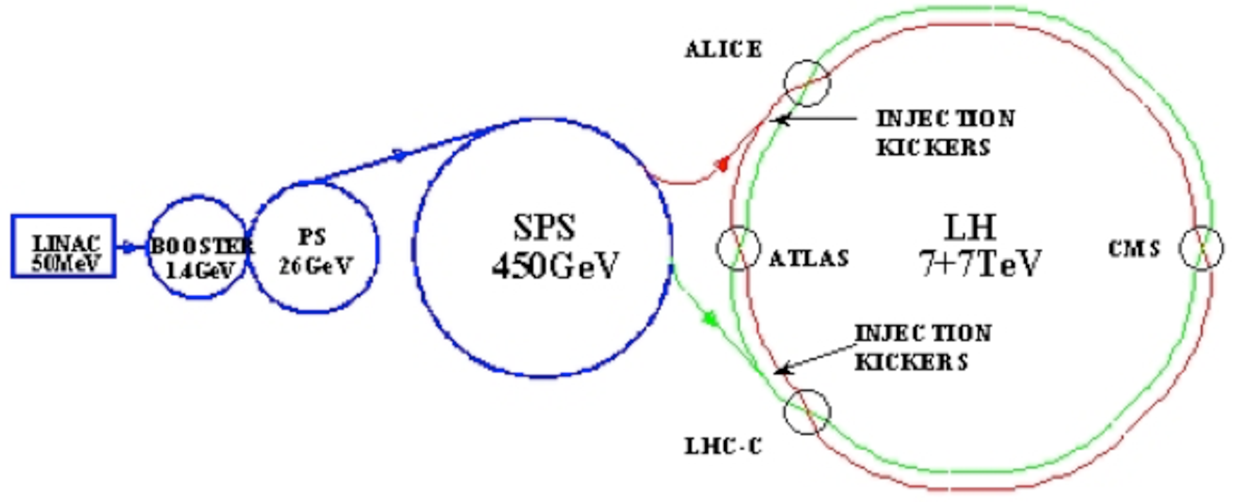
\includegraphics[scale=0.5]{./Particleaccelerators/Pictures/fig1.pdf}
\caption{Diagram of the CERN accelerator complex.}
\label{fig:pdgdedx}
\end{figure}

\section{Parts of an Accelerator}

Whether linear or circular, the basic parts of an accelerator are the same and are described below.

\;
\;
\;

\noindent
\textbf{Beam of particles for collisions}

\;
\;

\noindent
These are the particles that will be accelerated and then collided. LHC accelerates protons and heavy ions such as lead. For the LHC beam, 300 trillion protons are required, but since a single cubic centimetre of hydrogen gas at room temperature contains about 60 million trillion protons, the LHC can be refilled 200 000 times with just one cubic centimetre of gas - and it only needs refilling twice a day!

\;
\noindent
These protons are supplied from a hydrogen gas bottle. Hydrogen atoms consist of a proton and an electron. After stripping the hydrogen atom of its only electron we are left with a proton, which is then accelerated to required energy before colliding with protons accelerated in the opposite direction.

\;
\;

\begin{figure}[h]
\centering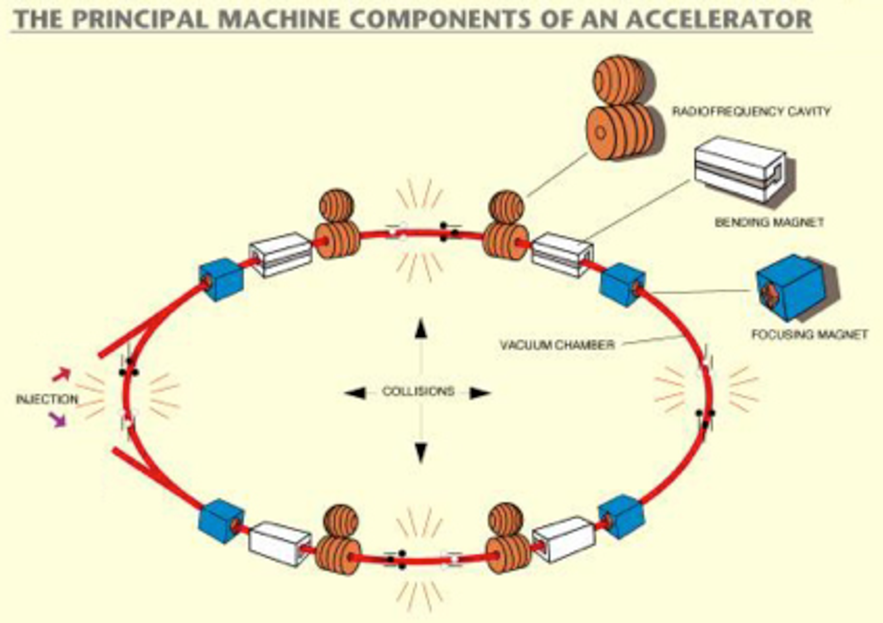
\includegraphics[scale=0.5]{./Particleaccelerators/Pictures/fig2.pdf}
\caption{Components of an Accelerator}
\label{fig:pdgdedx}
\end{figure}

\;
\;
\;

\noindent
\textbf{Beam Pipe}

\;
\;

\noindent 
This is a metal pipe inside which the beam of particles travels. For the LHC, we have two beam pipes for opposite traveling beams of particles. This pipe has to be empty of any other atoms (e.q., the one in air) to avoid collisions between gas molecules and the particles in the beam (Why is this a bad thing?). The pressure inside of the LHC is $ 10^{13}$ atm, ten times less then the pressure on The Moon.

\;
\;
\;

\noindent
\textbf{Devices to change particle speed (Radiofrequency (RF) cavitires and electric fields)}

\;
\;

\noindent
A radiofrequency (RF) cavity is a metallic cavity like structure that looks like beads around the beam pipe.  These cavities contain an electromagnetic field such that when charged particles pass through that field it transfers energy to these particles and they are pushed or accelerated forward along the accelerator. Think of a proton as a surfer riding a wave.  Every electromagnetic wave accelerates a bunch of particles, about 100 billion of them and each of the two beams consists of a number of such bunches, a few meters apart. These bunches are circulated in the beam pipe going around the LHC ring thousands of times per second. It takes about 20 minutes to get to the energies required and during that time the protons cover a distance further than from Earth to the Sun and back.

\;
\noindent
At full power, trillions of protons will race around the LHC accelerator ring 11,245 times a second, travelling at 99.99\% the speed of light. A motionless proton has a mass of 0.938 GeV (938 million electron volts).The accelerators bring them to a final mass (or energy, which in this case is practically the same thing) of 7000 billion electron volts (7 tera-eV or 7 TeV). If you could - hypothetically - accelerate a person of 100 kg in the LHC, his or her mass would end up being 700 t.

\;
\;
\;

\noindent
\textbf{Devices to change direction particle (Magnetic Fields)}

\;
\;

\noindent
Going back to our picnic on a hill, we can use gravity to accelerate us down but what if the steering stops working? Similarly, we can accelerate protons using electromagnetic force but in order to keep them in the circular path, the beam pipes are surrounded by a large magnet system that deflects the protons (recall protons are positively charged particles) The higher the speed of a particle, larger its mass becomes, and stronger magnets are need to steer it. This is where the limitations of a particle accelerator lie, since at a certain magnetic energy, the material of the magnetic coils cannot resist the forces of its own magnetic field anymore. 

\;
\noindent
The LHC uses various types of magnets to serve different functions. For example, dipole magnets are usually used to bend the path of a beam of particles that would otherwise travel in a straight line. Quadrupole magnets are used to focus a beam, gathering all the particles closer together (similar to the way that lenses are used to focus a beam of light). The magnets used in the LHC have been specially designed: the dominant part of the magnet system consists of 1232 dipole magnets, each with a length of about 16 m and a weight of 35 t, which can create a maximum magnetic field of 8.33 tesla - 150 000 stronger than Earths magnetic field.In addition to the dipole magnets, there are quadrupole magnets (with four magnetic poles) for focusing the beams, and thousands of additional smaller sextupole and octupole magnets (with six or eight magnetic poles each, respectively) for correcting the beam size and position. \textbf{How do you think the LHC uses the electromagnets to change the direction of the protons moving in the opposite direction in the beam pipe?}

\;
\noindent
All magnet coils and the accelerator cavities are built from special materials (niobium and titanium) that become superconducting at very low temperatures, conducting electricity to produce the electric and magnetic fields without resistance. To reach their maximum performance, the magnets need to be chilled to -271.3C (1.9K) - a temperature colder than outer space. To cool the magnets, much of the accelerator is connected to a distribution system of liquid nitrogen and helium (see box). Just one eighth of the LHCs cryogenic distribution system would qualify as the worlds largest firdge.

\;
\;
\;

\noindent
\textbf{Collision Targets}

\;
\;

\noindent
Collisions at accelerators can occur either against a fixed target, or between two beams of particles as is the case for LHC. Particle detectors are placed around the collision point to record and study the particles produced in these collisions.

\;
\noindent
Physicists will use the LHC to recreate the conditions just after the Big Bang, by colliding the two beams head-on at very high energy. Teams of physicists from around the world will analyse the particles created in the collisions using special detectors in a number of experiments dedicated to the LHC.Physicists will use the LHC to recreate the conditions just after the Big Bang, by colliding the two beams head-on at very high energy. Teams of physicists from around the world will analyse the particles created in the collisions using special detectors in a number of experiments dedicated to the LHC.


\section{Energy}


\noindent
The maximum design energy per beam for LHC 7 TeV (tera-electronvolt), corresponding to head-to-head collisions of 14 TeV.

\;
\;
\;

\begin{figure}[h]
\centering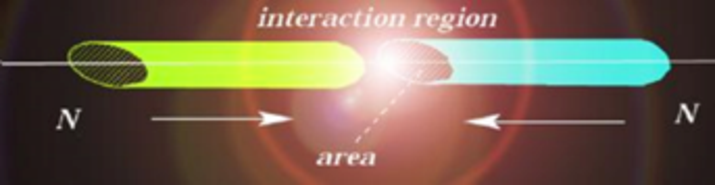
\includegraphics[scale=1.0]{./Particleaccelerators/Pictures/fig3.pdf}
\caption{Diagram of interaction region}
\label{fig:pdgdedx}
\end{figure}

\;
\;


\section{Cross Section}


\noindent
This is the transversal size of the bunch at the interaction point

\;
\;

\section{Luminosity (L)}


\noindent
Luminosity (L) is one of the most important parameters of an accelerator. Its a measurement of the number of collisions that can be produced in a detector per $cm^{2}$ and per second. The bigger the value of L is, the bigger the number of collisions. To calculate the number of collisions we need to also consider the cross section.

\begin{equation}\hspace{34 mm}L\sim f\cdot N^{2}/(4\cdot pi\cdot  \sigma ^{2}) = 10^{34} cm^{-2} \cdot s^{-1} \end{equation}

\;
\;

\noindent
Where f is the bunch's crossing frequency $40x10^{6}$. $N^{2}$ is the nymber of protons that can collide (each particle in a bunch might collide with anyone form the bunch approaching head on). And $\sigma$ is the cross section of the beam (=16 microns or $16\cdot 10^{-4}$).

\;
\;
\noindent
This value, $10^{34}cm^{-2}s^{-1}$, means that in the LHC might produce $10^{34}$ collisions per second, per $cm^{2}$. 

\;
\;

\section{Integrated Luminosity}

\noindent
This is the integral of the delivered luminosity over time. It is a measurement of the collected data size, and it is an important value to characterize the performance of an accelerator.

\begin{equation}\hspace{57 mm}L = \int L dt \end{equation}

\;
\;

\noindent
Usually, it is expresed as the inverse of cross section (i.e. 1/nb or nb$^{-1}$ - nanobarns$^{-1}$; 1/pb or pb$^{-1}$ - picobarn$^{-1}$; 1/fb or fb$^{-1}$ - femtobarn$^{-1}$)

\;
\;

\noindent Fig.5.4 shows the integrated luminosity (nb$^{-1}$) delivered to the LHC$'s$ experiments (3.5 TeV proton energies) through July 14 2010.

\;
\;

\begin{figure}[h]
\centering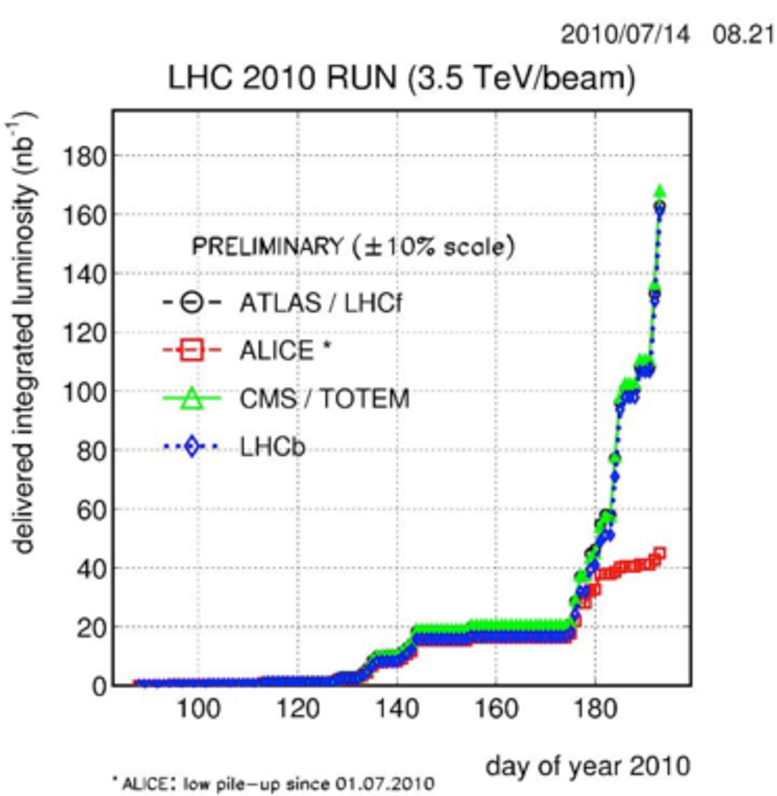
\includegraphics[scale=0.7]{./Particleaccelerators/Pictures/fig4.pdf}
\caption{Integrated Luminosity Through July 14 2010}
\label{fig:pdgdedx}
\end{figure}

\;
\;

\noindent
it is used by almost 10,000 physicists from more than 80 countries to search for particles to unravel the chain of events that shaped our Universe a fraction of a second after the Big Bang. It could resolve puzzles ranging from the properties of the smallest particles to the biggest structures in the vastness of the Universe. The design and construction of the LHC took about 20 years at a total cost of  3.6 billion euro. It is housed in a 27km long and 3.8m wide tunnel about 100m underground.

\;
\;

\noindent
\textbf{Given these parameters, how do you propose to increase the luminosity in a future LHC like machine?}

\;
\;

\section{Event}

\noindent
An event is a collision with all its resulting particles. In a ``damaging''  or hard collision, hundreds of particles, for example electrons, muons, photons, pions, protons, neutrons etc. Fly through the detector at close to the speed of light. These particles can come from the decay of heavier known or unknown particles and physicists use information collected by the detectors at different collision points to deduce the existence of these heavy particles. Multiple interactions??????

\;
\;

\section{The Data Challenge}

\noindent
The LHC will produce roughly 15 petabytes (15million gigabytes) of data annually - enough to fill more than 3 million DVDs.Thousands of scientists around the world want to access and analyse these data, so CERN is collaborating with institutions in 33 countries to operate a distributed computing and data storage infrastructure: The LHC Computing Grid (LCG)

\;
\;

\noindent
The LCG will allow data from the LHC experiments to be distributed around the globe, with a primary backup kept at CERN. After initial processing, the data will be distributed to eleven large computer centres. These tier-1 centres will make the data scientists can then access the LHC data from their home country, using local computer clusters or even individual PCs.

\;
\;

\section{Refrences}

\;

          $ \cdot \:$ An LHC FAQ PDF \url{http://cdsweb.cern.ch/record/1092437/files/CERN-Brochure-2008-001-Eng.pdf}

\;
\noindent
          $ \cdot \:$  A video of the HLC Rap \url{www.youtube.com/watch?v=j50ZssEojtM}

\;
\noindent
          $ \cdot \:$ The CERN$'s$ LHC public website \url{http://public.web.cern.ch/public/en/LHC}

\;
\noindent
          $ \cdot \:$ An online LHC game \url{http://microcosm.web.cern.ch/microcosm/LHCGame/LHCGame.html}


\;
